% Source: phaseTransitions_liquidCrystals.pdf, pages 7-20 (percolation and dilute spin models).
\subsection{Percolation and dilute spin models}
\subsubsection*{Lattice vacancies and percolation}

Another type of nonanalytic behavior has to do with lattice vacancies, defects, and impurities in real materials. These
can often be modelled by allowing sites to be occupied randomly with probability $p\in[0,1]$, and hence vacant with
probability $1-p$. This vacancy could describe, say, a nonmagnetic atom as an impurity (or dopant) in a magnetic material.
Alternatively, one can consider the case when the bonds are randomly present with probability $p$ or absent with
probability $1-p$. This can be of interest in describing the flow of a liquid through a porous medium (e.g.\ the flow of
water or oil through rock, relevant for oil prospecting). These are called site and bond ``percolation'' and spin models on
lattices with randomly vacant sites or bonds are called ``dilute'' spin models. Clearly as $p\to 0$, either for site or
bond percolation, there is no nontrivial thermodynamic limit. For example a lattice with randomly occupied bonds with
probability $p$, with $0<p<1$, might look like this (on a 2D lattice or a 2D slice of a 3D lattice):

\begin{diagram}
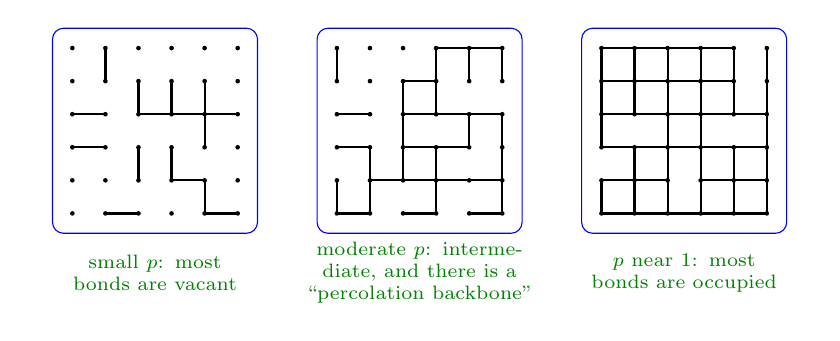
\begin{tikzpicture}[scale=0.42]
  \foreach \s/\pp/\seed/\lab in {0/0.2/11/{small $p$: most bonds are vacant},
                                  8/0.55/23/{moderate $p$: intermediate, and there is a ``percolation backbone''},
                                  16/0.9/37/{$p$ near 1: most bonds are occupied}} {
    \begin{scope}[xshift=\s cm]
      \pgfmathsetseed{\seed}
      \foreach \x in {0,...,5} \foreach \y in {0,...,5} {
        \fill (\x,\y) circle (0.07);
        \ifnum\x<5 \pgfmathparse{rnd<\pp ? 1 : 0}\ifnum\pgfmathresult=1 \draw[thick] (\x,\y) -- (\x+1,\y);\fi\fi
        \ifnum\y<5 \pgfmathparse{rnd<\pp ? 1 : 0}\ifnum\pgfmathresult=1 \draw[thick] (\x,\y) -- (\x,\y+1);\fi\fi
      }
      \draw[blue,rounded corners] (-0.6,-0.6) rectangle (5.6,5.6);
      \node[green!50!black,font=\scriptsize,align=center,text width=3cm] at (2.5,-1.8) {\lab};
    \end{scope}}
\end{tikzpicture}
\diagramcaption{Random bond occupation on a square lattice for small, moderate and large $p$.}
\end{diagram}

A basic question is whether, as $N\to\infty$, there is an infinite percolation backbone that extends from one side of the
lattice to the other. For the flow of a liquid like oil or water through rock, this determines whether the flow can take
place. For a spin model on the lattice, the existence of an infinite percolation backbone is a necessary condition for a
finite-temperature phase transition, since otherwise one just has spins interacting on finite clusters of sites and bonds,
and the associated finite sums $\sum_{\{s\}}e^{-\beta\Ham}$ are analytic.

For either site (s) or bond (b) percolation, on a lattice $\Lambda$ with dimension $d\ge 2$, as $p$ increases from 0 to 1,
there is a critical value $p_{c,\Lambda}^{(s)}$ or $p_{c,\Lambda}^{(b)}$ at which an infinite percolation backbone first
appears. This is a geometrical phenomenon, which can be studied purely as a function of $p^{(s)}$ or $p^{(b)}$ and
$\Lambda$, with no reference to temperature. One can also study the behavior of a spin model on a lattice $\Lambda$ with
site or bond vacancies. For a given type (site or bond) of vacancies and a given lattice $\Lambda$, one can define a
probability $P(p)$ that a given site is part of an infinite (connected) cluster. This serves as an order parameter for the
percolation transition:
\begin{equation}
  P(p)\propto(p-p_{c,\Lambda})^\beta\qquad\text{as } p-p_{c,\Lambda}\to 0^+ .
\end{equation}

\begin{diagram}
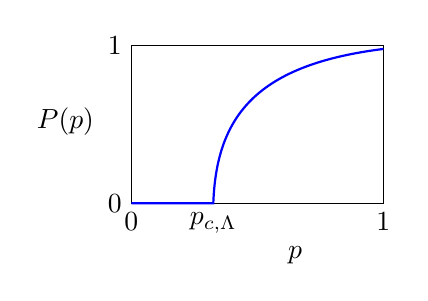
\begin{tikzpicture}[scale=0.8]
  \draw (0,0) rectangle (4,2.5);
  \draw[thick,blue] (0,0) -- (1.3,0) .. controls (1.35,1.4) and (2,2.2) .. (4,2.45);
  \node[left] at (0,2.5) {$1$}; \node[left] at (0,0) {$0$}; \node[left=10pt] at (0,1.3) {$P(p)$};
  \node[below] at (0,0) {$0$}; \node[below] at (4,0) {$1$}; \node[below] at (1.3,0) {$p_{c,\Lambda}$};
  \node[below=12pt] at (2.6,0) {$p$};
\end{tikzpicture}
\diagramcaption{The percolation order parameter.}
\end{diagram}

Thus $P(p)$ behaves nonanalytically as a function of $p$: $P(p) = 0$ for $0\le p\le p_{c,\Lambda}$ and $P(p)>0$ for
$p>p_{c,\Lambda}$. For example, $p_{c,sq}^{(b)} = 1/2$ for $\Lambda$ = square lattice (an exact value, from duality);
$p_{c,sq}^{(s)} = 0.59275$ (not known exactly; the value is from series and Monte Carlo simulations).

Series analyses and Monte Carlo simulations show that the critical exponent $\beta$ and other critical exponents
describing the percolation transition are the same for site and bond percolation and are independent of lattice type.
The critical percolation probabilities $p_{c,\Lambda}^{(s)}$ and $p_{c,\Lambda}^{(b)}$ do depend on site vs.\ bond
percolation and $\Lambda$. One can define an average cluster size, $S(p)$; as $p\nearrow p_{c,\Lambda}$, this diverges
and one writes $S(p)\propto(p_c-p)^{-\gamma}$ as $p\nearrow p_c$.

\paragraph{Connection to the Potts model.}

Bond percolation has an interesting connection to the Potts model. The average number of (connected) clusters on a
general graph $G$ defined by its vertex set $V$ and its edge (= bond) set $E$ is $\ev k$:
\begin{equation}
  \ev k = \frac{1}{n}\left[\sum_{G'\subseteq G}k(G')\,p^{e(G')}(1-p)^{e(G)-e(G')}\right]\Big/\left[\sum_{G'\subseteq G}p^{e(G')}(1-p)^{e(G)-e(G')}\right],
\end{equation}
where $G' = (V,E')$, $E'\subseteq E$, is a spanning subgraph, $k(G')$ is the number of connected clusters in $G'$,
$p^{e(G')}$ is the probability that all bonds of $G'$ are present, $(1-p)^{e(G)-e(G')}$ is the probability that all bonds
not on $G'$ are absent, and $n = n(G)$ = \# of vertices in $G$. Now recall that the cluster formula for the partition
function of the Potts model is
\begin{equation}
  Z(G,q,v) = \sum_{G'\subseteq G}q^{k(G')}v^{e(G')};
\end{equation}
set $v = v_b\equiv p/(1-p)$ (subscript b for bond) $\Rightarrow 0\le v_b\le\infty$, analogous to $v$ in the Potts
ferromagnet. Then
\begin{equation}
  Z(G,q,v_b) = \sum_{G'\subseteq G}q^{k(G')}p^{e(G')}(1-p)^{-e(G')}
  = (1-p)^{-e(G)}\sum_{G'\subseteq G}q^{k(G')}p^{e(G')}(1-p)^{e(G)-e(G')},
\end{equation}
so
\begin{equation}
  \frac{\partial\ln Z(G,q,v_b)}{\partial q}
  = \frac{\sum_{G'\subseteq G}k(G')q^{k(G')-1}p^{e(G')}(1-p)^{e(G)-e(G')}}{\sum_{G'\subseteq G}q^{k(G')}p^{e(G')}(1-p)^{e(G)-e(G')}},
\end{equation}
so
\begin{equation}
  \ev k = \frac{1}{n}\cdot\left.\frac{\partial\ln Z(G,q,v_b)}{\partial q}\right|_{q=1};\qquad
  \text{in the thermodynamic limit,}\quad \ev k = \left.\pder{f}{q}\right|_{q=1}
\end{equation}
(take $n\to\infty$ first, then take $q\to 1$); recall $f = \lim_{n\to\infty}(1/n)\ln Z$.

So the critical behavior of bond percolation is inferred to be the same as the $q\to 1$ limit of the $q$-state Potts
ferromagnet. This is also inferred to be true of the critical behavior of site percolation. In this $q\to 1$ limit in 2D,
the critical exponents are $\alpha = -2/3$, $\beta = 5/36 = 0.139$, $\gamma = 43/18 = 2.39$,
$\delta = 91/5 = 18.2$, $\eta = 5/24 = 0.208$, $\nu = 4/3$; $y_\tau = 1/\nu = 3/4$,
$y_h = 91/48$. These values have been confirmed by series analyses and Monte Carlo simulations. Recall the exact
value for the critical point of the $q$-state Potts FM on the square lattice is $v_c = \sqrt q$; here, this
$\Rightarrow(v_b)_c = p_c/(1-p_c) = \sqrt q = 1\Rightarrow p_{c,sq} = 1/2$ for bond percolation. In general,
$(p_c^{(s)})_\Lambda>(p_c^{(b)})_\Lambda$ for all $\Lambda$ except 1D, where $(p_c^{(s)})_{1D} = 1 = (p_c^{(b)})_{1D}$, and
$(p_c^{(s)})_\Lambda$ and $(p_c^{(b)})_\Lambda$ decrease with increasing $\Delta_\Lambda$.

Recall that $\lim_{n\to\infty}$ and $\lim_{q\to 1}$ do not commute. On a finite graph $G$, the Potts model Hamiltonian
evaluated at $q = 1$ is $\Ham = -J_Pe(G)$; $-\beta\Ham = Ke(G)$, so
$Z(G,q=1,v) = e^{Ke(G)} = (v+1)^{e(G)}$ (recall: $v = e^K-1$) and, e.g., for a $\Delta$-regular graph $G$,
$e(G) = (\Delta/2)n(G)$. So $Z(G,q=1,v) = (1+v)^{(\Delta/2)n}$ and
\begin{equation}
  f = \lim_{n\to\infty}\frac{1}{n}\ln Z = \frac{\Delta}{2}\ln(1+v) = \frac{\Delta}{2}\ln(e^K) = \frac{\Delta}{2}K;
\end{equation}
similarly for a general graph, $f = \left(\Delta_{\text{eff}}/2\right)K$, where
$\Delta_{\text{eff}} = \lim_{n\to\infty}(2e(G)/n(G))$. This is an analytic function of $K$, so the model evaluated for
$q = 1$ and then $n\to\infty$ has no critical behavior. The nontrivial critical behavior is obtained by taking $n\to\infty$
first and then $q\to 1$.

\paragraph{Properties of the average cluster number.}

The average cluster number $\ev k$ obtained in this limit has several general properties:
\begin{enumerate}[label=(\arabic*)]
  \item If $p = 0$, then no bonds are present, so each vertex is a cluster by itself. So \# clusters $= n$, and hence the
    average number of clusters per vertex is $n/n = 1$, so $\ev k = 1$. This is also evident from the definition of
    $\ev k$ with $p = 0$, so $v_p = p/(1-p) = 0$. Now $Z(G,q,v) = \sum_{G'\subseteq G}q^{k(G')}v^{e(G')}$, so the only
    contribution for $v = 0$ is from the spanning subgraph with no edges = bonds, $e(G') = 0$. This is the empty graph $E_n$
    with $n$ vertices, no bonds, and hence $n$ components, i.e.\ $k(E_n) = n$, so $Z(G,q,0) = q^n$; hence, $f = \ln q$,
    $\partial f/\partial q = 1/q$ and $\ev k = \left.\partial f/\partial q\right|_{q=1} = 1$ at $p = 0$.
  \item If $p = 1$, then there is only one cluster on $G$, namely $G$ itself. So the average cluster number as $n\to\infty$
    is $\ev k = \lim_{n\to\infty}(1/n) = 0$.
  \item As $p$ increases in the interval $0\le p\le 1$, the number of clusters decreases for a fixed $G$ and the number per
    vertex in the $n\to\infty$ limit also decreases, so $\ev k$ is a monotonically decreasing function of $p$ for
    $p\in[0,1]$, which decreases from $\ev k = 1$ at $p = 0$ to $\ev k = 0$ at $p = 1$.
  \item Increasing the vertex degree enhances connectivity of the vertices for a given $p$. Hence, the negative slope of
    $\ev k$ at $p = 0$, $\left.\dd\ev k/\dd p\right|_{p=0}$, increases in magnitude with $\Delta$. Specifically, one finds
    \begin{equation}
      \left.\frac{\dd\ev k}{\dd p}\right|_{p=0} = -\frac{\Delta}{2}
    \end{equation}
    for $\Delta$-regular lattice graphs, and $\left.\dd\ev k/\dd p\right|_{p=0} = -\Delta_{\text{eff}}/2$ more
    generally.
    One approaches the $\infty$ cluster more rapidly for larger $\Delta$ or $\Delta_{\text{eff}}$.
  \item Consider a strip graph $\Lambda_s$ of finite width $L_y$ and length $L_x = m$, with longitudinal boundary conditions
    BC$_x$ and transverse boundary conditions BC$_y$, e.g.\ free: (FBC$_x$, FBC$_y$); cyclic: (PBC$_x$, FBC$_y$);
    cylindrical: (FBC$_x$, PBC$_y$); toroidal: (PBC$_x$, PBC$_y$). In the limit $L_x\to\infty$ for fixed finite $L_y$,
    $f = \lim(1/n)\ln Z$ is independent of the longitudinal b.c.\ and depends on $L_y$ and BC$_y$, as well as the type of
    lattice (sq, tri, hc, etc.). Hence $\ev k = \left.\partial f/\partial q\right|_{q=1,v=v_p}$ has the same property. Thus we can label the
    result as $\ev k$ for $\Lambda$, $(L_y)_{BC_y}$, e.g.\ $\ev k$ for sq, $2_F$ or $2_P$, $3_F$ or $3_P$, etc.
\end{enumerate}

\begin{diagram}
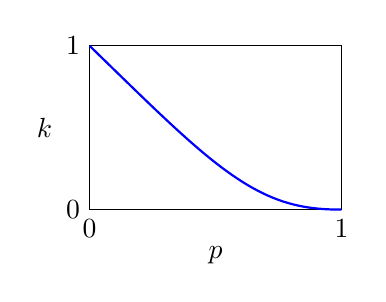
\begin{tikzpicture}[scale=0.8]
  \draw (0,0) rectangle (4,2.6);
  % the exact sq, 2_F strip result, <k> = (1-p)^2 (2+p-2p^2) / [2(1-p^2+p^3)]
  \draw[thick,blue,domain=0:1,samples=60,smooth] plot ({4*\x},{2.6*(1-\x)^2*(2+\x-2*\x^2)/(2*(1-\x^2+\x^3))});
  \node[left] at (0,2.6) {$1$}; \node[left] at (0,0) {$0$}; \node[left=10pt] at (0,1.3) {$\ev k$};
  \node[below] at (0,0) {$0$}; \node[below] at (4,0) {$1$}; \node[below=10pt] at (2,0) {$p$};
\end{tikzpicture}
\diagramcaption{Illustrative plot of $\ev k$ as a function of $p\in[0,1]$ for bond percolation on strip graphs with width
$L_y\ge 2$.}
\end{diagram}

Simplest example: $L_y = 1$: $Z = (q+v)^m + (q-1)v^m$. Since $v_p = p/(1-p)>0$, $f = \ln(q+v_p)$,
$\left.\partial f/\partial q\right|_{q=1} = 1/(1+v_p) = 1/(1+p/(1-p)) = (1-p)$, so $\ev k = 1-p$.

We have calculated $\ev k$ for a variety of different lattice strip graphs, e.g.\ (the result is independent of BC$_x$)
\begin{equation}
  \text{sq, }2_F\ (\text{FBC}_y):\quad \ev k = \frac{(1-p)^2(2+p-2p^2)}{2(1-p^2+p^3)},\qquad\Delta_{\text{eff}} = 3 .
\end{equation}
Taylor series expansion for small $p$:
\begin{equation}
  \ev k = 1-\frac{3}{2}p+\frac{1}{2}p^4+\frac{1}{2}p^6+\Order(p^7)\quad\text{for small }p,
\end{equation}
with the coefficient of $p$ equal to $-\Delta_{\text{eff}}/2$, so $\left.\dd\ev k/\dd p\right|_{p=0} = -3/2$. And
\begin{equation}
  \text{sq, }2_P:\quad \ev k = \frac{(1-p)^2(2-3p^2+2p^3)}{2(1+p-p^2)(1-p+p^2)}
\end{equation}
(S.-C.~Chang and R.~Shrock, Phys.\ Rev.\ E \textbf{70}, 056130 (2004)). The small-$p$ Taylor series expansion is
$\ev k = 1-2p+(1/2)p^2+2p^4+\Order(p^5)$.

For a given strip, $\ev k$ can equivalently be expressed as a function of $(1-p)\equiv r$, $r\in[0,1]$; e.g.
\begin{align}
  \text{sq, }2_F:&\quad \ev k = \frac{(1-p)^2(2+p-2p^2)}{2(1-p^2+p^3)} = \frac{r^2(1+3r-2r^2)}{2(1-r+2r^2-r^3)},\\
  &\quad\text{small-$r$ expansion: }\ev k_{2_F} = \frac{r^2}{2}+2r^3-\frac{7}{2}r^5+\Order(r^6),\nonumber\\
  \text{sq, }2_P:&\quad \ev k = \frac{r^2(1+3r^2-2r^3)}{2(1+r-r^2)(1-r+r^2)},\\
  &\quad\ev k_{2_P} = \frac{r^2}{2}+2r^4-2r^5+\Order(r^6).\nonumber
\end{align}
There is no known exact closed-form expression for $\ev k_\Lambda$ as a function of $p$ for any lattice $\Lambda$ of
dimension $d\ge 2$, so these exact analytic expressions are useful. As the strip width increases, the expressions for
$\ev k$ provide a progressively more accurate approximation to the (unknown) $\ev k$ function for the infinite 2D lattice.
A quantitative measure of this is how well the small-$p$ or small-$r$ Taylor series expansions match the corresponding
series expansions for the infinite 2D lattices. With a former Ph.D.\ thesis student, Shu-Chiuan Chang, we calculated
$\ev k$ for a variety of infinite-length, finite-width strip graphs of the sq, tri, and hc lattices and, from the
resulting exact expressions, computed small-$p$ and small-$r$ series expansions, in S.-C.~Chang and R.~Shrock, Phys.\ Rev.\
E \textbf{70}, 056130 (2004), op.\ cit.; J.\ Stat.\ Phys.\ \textbf{149}, 676 (2012); Phys.\ Rev.\ E \textbf{104}, 044107
(2021) [arXiv:2105.13415].

For a given type of lattice, the use of boundary conditions that minimize the effect of transverse boundaries (PBC$_y$)
yields faster approach to the series for $\ev k$ on infinite 2D lattices. For example, consider strips of the square
lattice. For the infinite square lattice,
\begin{equation}
  \ev k = 1-2p+p^4+2p^6-2p^7+\Order(p^8).
\end{equation}
With PBC$_y$, we calculate
\begin{align}
  2_P:&\quad \ev k = 1-2p+{\color{red}\frac{1}{2}p^2}+{\color{red}2p^4}-2p^5+\frac{5}{2}p^6+\Order(p^7),\\
  3_P:&\quad \ev k = 1-2p+{\color{red}\frac{1}{3}p^3}+p^4+{\color{red}2p^5}+\Order(p^7),\\
  4_P:&\quad \ev k = 1-2p+{\color{red}\frac{5}{4}p^4}+{\color{red}5p^6}+\Order(p^7),\\
  5_P:&\quad \ev k = 1-2p+p^4+\frac{1}{5}p^5+2p^6+\Order(p^7),\quad\text{etc.}
\end{align}
(terms that differ from the infinite-lattice series are in red). Similar results hold for the small-$r$ series and other
lattices.

\paragraph{Complex singularities of the average cluster number.}

Another interesting output of these exact calculations of $\ev k$ for infinite-length, finite-width lattice strips is the
singularities of $\ev k$ in the complex $p$ plane. We prove that $\ev k$ is a rational function of $p$, so its
singularities are poles. For example,
\begin{equation}
  \text{sq, }2_F:\quad \ev k = \frac{(1-p)^2(2+p-2p^2)}{2(1-p^2+p^3)}
\end{equation}
has poles at $p = -0.754878$ and $p = 0.877439\pm 0.744862\,\ii$ (magnitude 1.15096), and
\begin{equation}
  \text{sq, }2_P:\quad \ev k = \frac{(1-p)^2(2-3p^2+2p^3)}{2(1+p-p^2)(1-p+p^2)}
\end{equation}
has poles at $p = (1/2)(1\pm\sqrt3\,\ii)$, magnitude $|p| = 1$, and at
$p = (1/2)(1+\sqrt5) = 1.61803$ and $p = (1/2)(1-\sqrt5) = -0.61803$, and so forth for other strips.

The poles nearest to the origin determine the radius of convergence of the small-$p$ Taylor series. It was previously
observed that the radius of convergence of the small-$p$ series for $\ev k$ on 2D lattices can be smaller than $p_c$, the
critical percolation probability. For example for the square lattice, $p_c = 1/2$. Recall that the critical point of the
Potts model for $v>0$ (FM $J>0$) is given by $v_c = \sqrt q$, so $v_c = 1$, and since $v_p = p/(1-p)$ for bond
percolation, $v_c = 1\Leftrightarrow p_c = 1/2$. But series analyses found that the radius of convergence is $\sim 0.4$,
smaller than $p_c$. Our results explain this, as is shown by a table of the distances of the nearest poles to the origin
from $p = 0$:
\begin{center}
\begin{tabular}{lc}
  strip & $|p|$, pole closest to origin\\ \hline
  sq, $2_P$ & 0.618\\
  sq, $3_P$ & 0.478\\
  sq, $4_P$ & 0.424\\
  sq, $5_P$ & 0.409
\end{tabular}
\end{center}
and similarly for other lattices. See the tables in Chang and Shrock, Phys.\ Rev.\ E \textbf{104}, 044107 (2021),
arXiv:2105.13415 for more details.

Percolation continues to be a subject of considerable interest in statistical mechanics and condensed matter physics, as
well as in engineering and applied physics.

\paragraph{Example of a calculation: the square-lattice ladder.}

Consider the square-lattice ladder graph with FBC$_y$. As above, this is denoted $[\text{sq},2_F]$. The result for $\ev k$
is independent of the longitudinal b.c., BC$_x$. Let us take PBC$_x$. Denote a strip of length $m$ vertices as
$L_m$, sq$_{2_F}$ ($L$ for ladder). In R.~Shrock, Physica \textbf{283}, 388 (2000), we calculated $Z(L_m,q,v)$:
\begin{equation}
  Z(L_m,q,v) = \left(\lambda_{2,0,1}^m+\lambda_{2,0,2}^m\right) + (q-1)\left[\lambda_{2,1,1}^m+\lambda_{2,1,2}^m+\lambda_{2,1,3}^m\right]
             + (q^2-3q+1)\lambda_{2,2,1}^m,
\end{equation}
where
\begin{align}
  \lambda_{2,0,(1,2)} &= \frac{1}{2}\left[T_{S0}\pm\sqrt{R_{S0}}\right],\qquad T_{S0} = v^3+4v^2+3qv+q^2,\nonumber\\
  R_{S0} &= v^6+4v^5-2qv^4-2q^2v^3+12v^4\nonumber\\ &\quad+16qv^3+13q^2v^2+6q^3v+q^4,\nonumber\\
  \lambda_{2,1,(1,2)} &= \frac{v}{2}\left[T_{S1}\pm\sqrt{R_{S1}}\right],\qquad T_{S1} = q+v(v+4),\nonumber\\
  R_{S1} &= v^4+4v^3+12v^2-2qv^2+4qv+q^2,\nonumber\\
  \lambda_{2,1,3} &= v(v+q),\qquad \lambda_{2,2,1} = v^2;
\end{align}
the number of vertices is $n = L_yL_x = 2m$. Then
\begin{equation}
  f = \lim_{n\to\infty}\frac{1}{n}\ln Z = \frac{1}{2}\ln\lambda_{\text{dominant}} .
\end{equation}
In the region of interest here, $q\to 1$, $v = p/(1-p)$ with $p\in[0,1]$, so $v\ge 0$, and the dominant $\lambda$ is
$\lambda_{2,0,1}$. Then
\begin{equation}
  \ev k = \left.\pder{f}{q}\right|_{q=1} = \left.\frac{1}{2}\lambda_{\text{dom}}^{-1}\frac{\partial\lambda_{\text{dom}}}{\partial q}\right|_{q=1}.
\end{equation}
An elegant way to do this calculation is to use the fact that $\lambda_{2,0,(1,2)}$ are roots of a quadratic equation:
\begin{equation}
  \lambda^2 - (v^3+4v^2+3qv+q^2)\lambda + v^2(v+1)(v+q)^2 = 0,
\end{equation}
so
\begin{equation}
  2\lambda\pder{\lambda}{q} - (v^3+4v^2+3qv+q^2)\pder{\lambda}{q} - (3v+2q)\lambda + v^2(v+1)(2v+2q) = 0
\end{equation}
\begin{equation}
  \Rightarrow\quad\pder{\lambda}{q} = \left[(3v+2q)\lambda - 2v^2(v+1)(v+q)\right]\Big/\left[2\lambda - (v^3+4v^2+3qv+q^2)\right].
\end{equation}
Now, for a general $G$, at $q = 1$, $Z(G,1,v) = e^{Ke(G)} = (v+1)^{e(G)}$, with $e(G)$ = \# of edges in $G$; for a
$\Delta$-regular graph $G$, $e(G) = (\Delta/2)n = \Delta/2\cdot mL_y$, where $n = mL_y$, so
\begin{align}
  f(G,q=1,v) &= \lim_{m\to\infty}\frac{1}{n}\ln Z = \frac{1}{n}\ln\lambda_{\text{dom}}^m = \frac{1}{L_y}\ln\lambda_{\text{dom}}\nonumber\\
  &= \frac{\Delta}{2}\ln(v+1)\ \Rightarrow\ (\lambda_{\text{dom}})^{1/L_y} = (1+v)^{\Delta/2},
\end{align}
i.e.\ $\lambda_{\text{dom}}(G,q=1) = (1+v)^{(\Delta/2)L_y}$. Setting $v = v_p = p/(1-p)\Rightarrow
1+v = 1+p/(1-p) = 1/(1-p)$, so $\lambda_{\text{dom}}(G,q=1,v=v_p) = \left(1/(1-p)\right)^{(\Delta/2)L_y}$. For the
square ladder strip, $\Delta = 3$, $L_y = 2$, so $\lambda_{\text{dom}}(L_m,q=1,v=v_p) = \left(1/(1-p)\right)^3$. So
\begin{equation}
  \ev k = \left.\pder{f}{q}\right|_{q=1} = \left.\frac{1}{L_y}\frac{\partial\lambda_{\text{dom}}/\partial q}{\lambda_{\text{dom}}}\right|_{q=1}.
\end{equation}
Substituting the above value of $\lambda_{\text{dom}}$ at $q = 1$, $v = v_p$ in this expression and evaluating our result
above for $\left.\partial\lambda_{\text{dom}}/\partial q\right|_{q=1}$ at $v = v_p$, we finally obtain the solution for
$\ev k$ for the $L_x\equiv m\to\infty$ limit of this sq, $2_F$ strip, namely
\begin{equation}
  \ev k_{\text{sq},2_F} = \frac{(1-p)^2(2+p-2p^2)}{2(1-p^2+p^3)}.
\end{equation}

\paragraph{Site versus bond percolation thresholds.}

It is easy to see why $(p_c^{(s)})_{1D} = (p_c^{(b)})_{1D} = 1$ on the 1D lattice: if $p<1$, then sites or bonds may be
absent, but then this would prevent the existence of a path connecting a site to the left of the break to a site to the
right of the break.

On a higher-dimensional lattice, removing a site causes a greater reduction in the pathways than removing a bond, e.g.\ on a
square lattice: removing a site also renders the adjacent bonds unusable, while removing a bond leaves the adjacent sites
still usable. So it is necessary to have a higher occupation probability $p$ to get an $\infty$ percolation cluster for site
percolation than for bond percolation: $(p_c^{(s)})_\Lambda>(p_c^{(b)})_\Lambda$, $\Lambda>1D$.

\begin{diagram}
\begin{tikzpicture}[scale=0.4,>=Stealth]
  % (a) a site marked for removal, (b) the lattice without it and its four bonds
  \foreach \x in {0,...,4} \draw[blue] (\x,-0.4) -- (\x,4.4);
  \foreach \y in {0,...,4} \draw[blue] (-0.4,\y) -- (4.4,\y);
  \fill[red] (2,2) circle (0.18);
  \draw[red,thick] (1.5,1.7) -- (1.5,2.3); \draw[red,thick] (2.5,1.7) -- (2.5,2.3);
  \draw[red,thick] (1.7,1.5) -- (2.3,1.5); \draw[red,thick] (1.7,2.5) -- (2.3,2.5);
  \draw[->] (4.9,2) -- (6.3,2);
  \begin{scope}[xshift=6.8cm]
    \foreach \x in {0,1,3,4} \draw[blue] (\x,-0.4) -- (\x,4.4);
    \foreach \y in {0,1,3,4} \draw[blue] (-0.4,\y) -- (4.4,\y);
    \draw[blue] (2,-0.4) -- (2,1); \draw[blue] (2,3) -- (2,4.4);
    \draw[blue] (-0.4,2) -- (1,2); \draw[blue] (3,2) -- (4.4,2);
  \end{scope}
  \node[red,font=\scriptsize,align=center,text width=4.6cm] at (5.6,-1.6) {removing the site, which also renders the adjacent bonds unusable};
  % (c) a bond marked for removal, (d) the lattice without it
  \begin{scope}[xshift=14.5cm]
    \foreach \x in {0,...,4} \draw[blue] (\x,-0.4) -- (\x,4.4);
    \foreach \y in {0,...,4} \draw[blue] (-0.4,\y) -- (4.4,\y);
    \draw[red,very thick] (1.5,1.7) -- (1.5,2.3);
    \draw[->] (4.9,2) -- (6.3,2);
  \end{scope}
  \begin{scope}[xshift=21.3cm]
    \foreach \x in {0,...,4} \draw[blue] (\x,-0.4) -- (\x,4.4);
    \foreach \y in {0,1,3,4} \draw[blue] (-0.4,\y) -- (4.4,\y);
    \draw[blue] (-0.4,2) -- (1,2); \draw[blue] (2,2) -- (4.4,2);
  \end{scope}
  \node[red,font=\scriptsize,align=center,text width=4.6cm] at (20.1,-1.6) {removing a bond, but the adjacent sites are still usable};
\end{tikzpicture}
\diagramcaption{Removing a site on the square lattice removes four bonds; removing a bond removes one.}
\end{diagram}

Inequalities: $p_{c,\Lambda}^{(s)}>p_{c,\Lambda}^{(b)}$ for $\Lambda>1D$ (so sq, tri, hc, sc, etc.); $p_{c,\Lambda}^{(s)}$ and
$p_{c,\Lambda}^{(b)}$ are monotonically decreasing functions of the coordination number (vertex degree) of $\Delta$-regular
lattices $\Lambda$. These inequalities are evident in the values of $p_{c,\Lambda}^{(s)}$ and $p_{c,\Lambda}^{(b)}$ for known
cases. These values are known numerically from analysis of series expansions and from Monte Carlo simulations, and in certain
cases are known exactly.
\begin{center}
\begin{tabular}{lcccc}
  $\Lambda$ & $\Delta_\Lambda$ & $p_{c,\Lambda}^{(s)}$ & $p_{c,\Lambda}^{(b)}$ & \\ \hline
  1D & 2 & 1 & 1 & $d = 1$\\ \hline
  hc & 3 & 0.697 & 0.653 & \\
  sq & 4 & 0.593 & 0.5 & $d = 2$\\
  tri & 6 & 0.5 & 0.347 & \\ \hline
  sc & 6 & 0.312 & 0.249 & \\
  bcc & 8 & 0.246 & 0.180 & $d = 3$\\
  fcc & 12 & 0.199 & 0.120 &
\end{tabular}
\end{center}
As discussed above, the percolation threshold probability $p_{c,\Lambda}^{(s)}$ for site percolation and
$p_{c,\Lambda}^{(b)}$ for bond percolation is the analogue for the percolation transition of the critical temperature
$T_{c,\Lambda}$ for a thermal transition, in that the order parameter $P(p) = 0$ for $p<p_{c,\Lambda}$ and $P(p)>0$ for
$p>p_{c,\Lambda}$ for site or bond percolation, with $P(p)\sim(p-p_{c,\Lambda})^\beta$ as $p-p_{c,\Lambda}\to 0^+$, where
$P(p)$ is the probability that a given site is a member of an infinite cluster. Series analyses and Monte Carlo simulations
support the conclusion that critical exponents such as $\beta$ are the same for site and bond percolation and are also
independent of lattice type in a fixed spatial dimension $d$ (e.g.\ sq, tri, hc in $d = 2$, etc.), but do depend on $d$.

\paragraph{Cluster sizes and correlations.}

Let us denote a cluster containing $s$ sites as an $s$-cluster. As we denoted the average cluster number per site
(including all $s$ values) as $\ev k$ (often written as $\ev n$ in the percolation literature), let us also write the
average number of $s$-clusters per site as $\ev k_s$. Since a site can be any of the sites on an $s$-cluster, the probability
that a given site is a member of an $s$-cluster is $s\ev k_s$. Let us discuss cluster size in the case of site percolation;
an analogous discussion holds for bond percolation. The probability that a site belongs to some $s$-cluster for any $s$ is
$\sum_{s=1}^\infty s\ev k_s$, which is equal to the probability that this site is occupied, so
\begin{equation}
  \sum_{s=1}^\infty s\ev k_s = p .
\end{equation}
The average cluster size $S(p)$ can be related to $\ev k_s$ as follows. Since the probability that a given site is on an
$s$-cluster is $s\ev k_s$ and the probability that it belongs to any cluster is $\sum_ss\ev k_s$, the probability that the
cluster to which the site belongs contains $s$ sites is
\begin{equation}
  w_s = \frac{s\ev k_s}{\sum_ss\ev k_s}.
\end{equation}
Therefore the average cluster size is
\begin{equation}
  S = S(p) = \sum_ssw_s = \frac{\sum_ss^2\ev k_s}{\sum_ss\ev k_s}.
\end{equation}
As $p$ approaches $p_c$ from below, i.e.\ $p\nearrow p_c$, $S(p)\nearrow\infty$, $S(p)\sim(p_c-p)^{-\gamma}$. If one
subtracts the $\infty$ cluster present for $p>p_c$, then one also finds that $S(p)\sim|p-p_c|^{-\gamma}$ for $p\searrow p_c$.
In thermal phase transitions, one distinguished $\gamma$, $\gamma'$ for $\chi\sim(T-T_c)^{-\gamma}$, $T-T_c\to 0^+$ and
$\chi\sim(T_c-T)^{-\gamma'}$, $T-T_c\to 0^-$, but since equalities $\gamma = \gamma'$ etc.\ were established for thermal phase
transitions and were also found for percolation, one usually just writes $\gamma$, etc.

The pair correlation function, commonly denoted $g(r)$ or $C(r)$, is the probability, given one (occupied) site, that it is
connected with another site a distance (in lattice units) $r$ away, i.e.\ that they are members of the same cluster. For
$p\ne p_c$, this has a dominant exponential decay for large $r$:
\begin{equation}
  C(r)\sim e^{-r/\xi},
\end{equation}
where the correlation length is $\xi$. This is analogous to the spin--spin correlation function in a magnetic system, with
$T<T_c$ corresponding to $p>p_c$ as the more ordered regime and $T>T_c$ corresponding to $p<p_c$ as the less ordered regime.
Just as one subtracts the spontaneous magnetization squared from the spin--spin correlation function for $T<T_c$, so one
subtracts the infinite cluster's contribution to $C(r)$ in the percolation case. As $p\nearrow p_c$, $\xi\to\infty$ and, with
the above-mentioned subtraction, also as $p\searrow p_c$, $\xi\to\infty$, as
\begin{equation}
  \xi\sim\frac{1}{|p-p_c|^\nu}.
\end{equation}
The correlation length characterizes the length scale of a typical cluster, so the fact that it diverges at $p = p_c$ is
equivalent to the divergence in the average cluster size $S$. At $p = p_c$, $C(r)$ has the scaling behavior
$C(r)\sim1/r^{d-2+\eta}$, again similar to the spin--spin correlation function in a magnetic system at $T = T_c$,
where $\eta$ is the associated critical exponent.

The average number of clusters with $s$ sites, $\ev k_s$, behaves for large $s$ as
\begin{equation}
  \ev k_s\sim s^{-\tau}e^{-s/s_0},
\end{equation}
where $s_0$ measures the value of $s$ where the behavior changes from power-law decrease to exponential decrease. As
$p\to p_c$, $s_0\to\infty$ as $s_0\sim|p-p_c|^{-1/\sigma}$. At $p = p_c$, $\ev k_s\sim s^{-\tau}$ for large $s$. The critical
exponents $\sigma$ and $\tau$ thus determine the behavior of $\ev k_s$ (commonly written as $n_s$), the average number of
$s$-clusters per site, as a function of $p$.

Concerning the average number of clusters per site, although this is finite at $p = p_c$, it is non-analytic; since it is
related to the reduced free energy for the $q = 1$ Potts model, and since $f_{\text{sing}}\sim|T-T_c|^{2-\alpha}$ as
$T\to T_c$, so (2nd derivative with respect to $T$) $C_{\text{sing}}\sim|T-T_c|^{-\alpha}$, analogously, one has
$\ev k_{\text{sing}}\sim|p-p_c|^{2-\alpha}$.

\begin{center}
\renewcommand{\arraystretch}{1.25}
\begin{tabular}{lcc}
  crit.\ exp. & $d = 2$ & $d = 3$\\ \hline
  $\alpha$ & $-2/3 = -0.667$ & $-0.63$\\
  $\beta$ & $5/36 = 0.139$ & 0.42\\
  $\gamma$ & $43/18 = 2.39$ & 1.8\\
  $\nu$ & $4/3 = 1.33$ & 0.88\\
  $\eta$ & $5/24 = 0.208$ & $-0.03$\\
  $\delta$ & $91/5 = 18.2$ & 5.2\\
  $\sigma$ & $36/91 = 0.396$ & 0.45\\
  $\tau$ & $187/91 = 2.055$ & 2.19
\end{tabular}

\smallskip
{\small Values of critical exponents in percolation ($d = 3$ values are approximate).}
\end{center}

\paragraph{Fractal structure of the incipient infinite cluster.}

An interesting feature of percolation is that, as computer simulations have shown, at $p_c$ ($p_{c,\Lambda}^{(s)}$ or
$p_{c,\Lambda}^{(b)}$ for site or bond percolation on a lattice $\Lambda$) the incipient infinite percolation cluster has a
highly ramified structure. In the $N\to\infty$ limit, this incipient infinite percolation cluster is self-similar, i.e.\ has
the same structure when viewed on different length scales that are $\gg$ lattice spacing. It is thus a fractal, with a
Hausdorff dimension $d_H = d_f$ that is non-integral.

Recall the definition of the Hausdorff dimension. The idea is that if one increases the volume by a factor $b$, then the
number of relevant units of the entity changes by $N\sim b^{d_H}$, so $\ln N\sim d_H\ln b$,
\begin{equation}
  \Rightarrow\quad d_H = \frac{\ln N}{\ln b}.
\end{equation}
For example, with $b = 2$, one square $\to$ four squares, $N = 1\to N = 4$, so $d_H = \ln 4/(\ln 2) = 2\ln 2/(\ln 2) = 2$.
This shows that the Hausdorff dimension is 2, equal to the usual geometrical dimension, 2, of $\mathbb R^2$, the plane. Note
that this does not depend on how we tile the plane; for example consider tiling with triangles: with $b = 2$, $N = 1$ triangle
$\to$ 4 triangles, so $d_H = \ln N/(\ln b) = \ln 4/(\ln 2) = 2$, the same as with squares.

But now consider a different type of iterated procedure, in which, at each step, we remove one of the areas. To indicate this we
use color for the areas that are retained. For example, consider the ``Sierpinski gasket'', defined as the limit $m\to\infty$ of
the iterated process:

\begin{diagram}
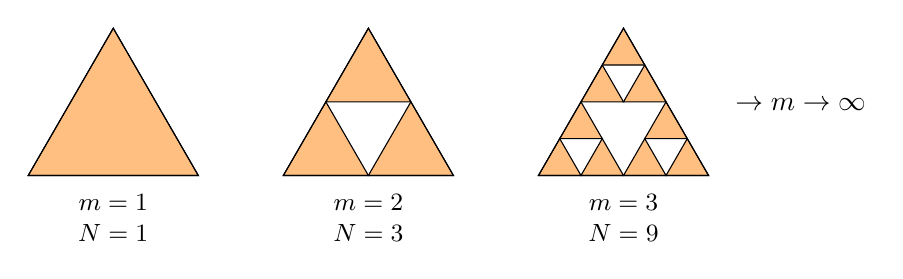
\begin{tikzpicture}[scale=0.9]
  \fill[orange!50] (0.000,0.000) -- (2.400,0.000) -- (1.200,2.078) -- cycle; \draw (0.000,0.000) -- (2.400,0.000) -- (1.200,2.078) -- cycle;
  \draw (0.000,0) -- (2.400,0) -- (1.200,2.078) -- cycle;
  \node[font=\small,align=center] at (1.2,-0.6) {$m = 1$\\ $N = 1$};
  \fill[orange!50] (3.600,0.000) -- (4.800,0.000) -- (4.200,1.039) -- cycle; \draw (3.600,0.000) -- (4.800,0.000) -- (4.200,1.039) -- cycle;
  \fill[orange!50] (4.800,0.000) -- (6.000,0.000) -- (5.400,1.039) -- cycle; \draw (4.800,0.000) -- (6.000,0.000) -- (5.400,1.039) -- cycle;
  \fill[orange!50] (4.200,1.039) -- (5.400,1.039) -- (4.800,2.078) -- cycle; \draw (4.200,1.039) -- (5.400,1.039) -- (4.800,2.078) -- cycle;
  \draw (3.600,0) -- (6.000,0) -- (4.800,2.078) -- cycle;
  \node[font=\small,align=center] at (4.8,-0.6) {$m = 2$\\ $N = 3$};
  \fill[orange!50] (7.200,0.000) -- (7.800,0.000) -- (7.500,0.520) -- cycle; \draw (7.200,0.000) -- (7.800,0.000) -- (7.500,0.520) -- cycle;
  \fill[orange!50] (7.800,0.000) -- (8.400,0.000) -- (8.100,0.520) -- cycle; \draw (7.800,0.000) -- (8.400,0.000) -- (8.100,0.520) -- cycle;
  \fill[orange!50] (7.500,0.520) -- (8.100,0.520) -- (7.800,1.039) -- cycle; \draw (7.500,0.520) -- (8.100,0.520) -- (7.800,1.039) -- cycle;
  \fill[orange!50] (8.400,0.000) -- (9.000,0.000) -- (8.700,0.520) -- cycle; \draw (8.400,0.000) -- (9.000,0.000) -- (8.700,0.520) -- cycle;
  \fill[orange!50] (9.000,0.000) -- (9.600,0.000) -- (9.300,0.520) -- cycle; \draw (9.000,0.000) -- (9.600,0.000) -- (9.300,0.520) -- cycle;
  \fill[orange!50] (8.700,0.520) -- (9.300,0.520) -- (9.000,1.039) -- cycle; \draw (8.700,0.520) -- (9.300,0.520) -- (9.000,1.039) -- cycle;
  \fill[orange!50] (7.800,1.039) -- (8.400,1.039) -- (8.100,1.559) -- cycle; \draw (7.800,1.039) -- (8.400,1.039) -- (8.100,1.559) -- cycle;
  \fill[orange!50] (8.400,1.039) -- (9.000,1.039) -- (8.700,1.559) -- cycle; \draw (8.400,1.039) -- (9.000,1.039) -- (8.700,1.559) -- cycle;
  \fill[orange!50] (8.100,1.559) -- (8.700,1.559) -- (8.400,2.078) -- cycle; \draw (8.100,1.559) -- (8.700,1.559) -- (8.400,2.078) -- cycle;
  \draw (7.200,0) -- (9.600,0) -- (8.400,2.078) -- cycle;
  \node[font=\small,align=center] at (8.4,-0.6) {$m = 3$\\ $N = 9$};
  \node at (10.9,1) {$\to m\to\infty$};
\end{tikzpicture}
\diagramcaption{Construction of the Sierpinski gasket ($b = 2$). The $m = \infty$ object is self-similar, a ``fractal'' with
non-integral dimension.}
\end{diagram}

Then
\begin{equation}
  d_H = \frac{\ln N}{\ln b} = \frac{\ln 3}{\ln 2} = 1.585 .
\end{equation}
The Hausdorff dimension is less than 2, as one expects, since at each iteration, some area is removed.

One can also model the fractal dimension of the percolation by writing $M\sim\ell^{d_f}$, where $\ell$ is a characteristic
length of the growing cluster as $p\to p_c$ and $M$ is proportional to the \# sites in this cluster. Computer simulations
yield $d_f = 1.89$ for $d = 2$ and $d_f = 2.53$ for $d = 3$, for both site and bond percolation. The ramification is
reflected in the property that $d_f<d$. Experimental realizations of fractals include, e.g., diffusion-limited aggregation,
DLA.

In addition to the flow of oil and water through a porous medium such as rock, percolation theory has also been applied to
other phenomena, e.g.\
(1) the spread of forest fires, using site percolation, with an occupied site representing a burning tree, and $p_c$ being the
critical probability that the fire will spread out of control;
(2) disease epidemics; the site percolation model would set $p$ = probability that an individual is infected by the disease and
hence can spread it.

\subsubsection*{Dilute spin models}

An important related topic is spin models in media with
\begin{enumerate}[label=(\roman*)]
  \item lattice vacancies at sites or crystal imperfections leading to missing bonds, or both;
  \item impurities, e.g.\ non-magnetic atoms as impurities in a magnetic material such as iron;
  \item deliberate ``doping'': addition of different types of atoms to obtain some desired property, such as adding carbon to
    iron to get steel, which is stronger than pure iron.
\end{enumerate}
As the site or bond occupation probability decreases from 1, the critical temperature decreases from its value for the
undiluted lattice $\Lambda$. As $p\searrow p_{c,\Lambda}^{(s)}$ for site vacancies or $p\searrow p_{c,\Lambda}^{(b)}$ for
bond vacancies, there is no longer an infinite cluster of sites. Then, since $Z = \sum e^{-\beta\Ham}$ is a finite sum, there
is no nonanalytic behavior: no phase transition at any finite temperature. A typical plot of $T_c(p)/T_c(1)$ for either site
or bond dilution is:

\begin{diagram}
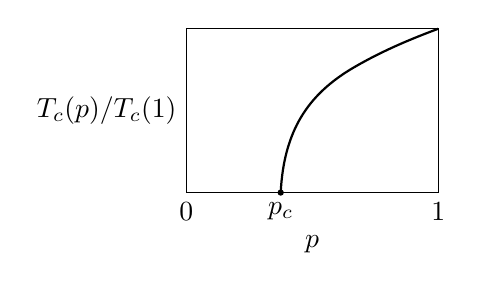
\begin{tikzpicture}[scale=0.8]
  \draw (0,0) rectangle (4,2.6);
  \draw[thick] (1.5,0) .. controls (1.55,1.0) and (1.95,1.55) .. (2.6,1.95) .. controls (3.1,2.25) and (3.6,2.45) .. (4,2.6);
  \fill (1.5,0) circle (0.05);
  \node[below] at (0,0) {$0$}; \node[below] at (1.5,0) {$p_c$}; \node[below] at (4,0) {$1$}; \node[below=12pt] at (2,0) {$p$};
  \node[left] at (0,1.3) {$T_c(p)/T_c(1)$};
\end{tikzpicture}
\diagramcaption{Critical temperature of a dilute spin model as a function of the occupation probability.}
\end{diagram}

For further information on percolation and dilute spin models, see, e.g.:
\begin{itemize}
  \item J.~Essam, Rept.\ Prog.\ Phys.\ \textbf{43}, 833 (1980);
  \item D.~Stauffer and A.~Aharony, \emph{Introduction to Percolation Theory} (2nd ed.\ 1991);
  \item R.~Stinchcombe, in vol.~7 of C.~Domb and J.~Lebowitz, \emph{Phase Transitions and Critical Phenomena} (1983).
\end{itemize}
Mathematical treatments include G.~Grimmett, \emph{Percolation} (1999); B.~Bollob\'as and O.~Riordan, \emph{Percolation}
(2006). On fractals, see, e.g., B.~Mandelbrot, \emph{The Fractal Geometry of Nature} (1982).
